%!TEX root = ../../../adrien_gomar_phd.tex

\subsection{Using the prediction tool}
\label{sub:dream_hs_conv_hb_prediction_tool}

The prediction tool developed in Chap.~\ref{cha:limitations_convergence}
is used to estimate the number of harmonics needed to compute
this high-speed configuration.
Seven harmonics are required to capture 99\% of the energy
(Fig.~\ref{fig:DREAM_HS_RANS_ROE2_SPECTRUM_PPT}).
\begin{figure}[htp]
  \centering
  \includegraphics*[width=0.5\textwidth]{DREAM_HS_RANS_ROE2_SPECTRUM_PPT.pdf}
  \caption{High-speed isolated configuration: prediction of the number
  of harmonics needed to simulate the configuration.}
  \label{fig:DREAM_HS_RANS_ROE2_SPECTRUM_PPT}
\end{figure}

In the following, the $N=7$ HB computation will be
considered to be converged and therefore used to 
analyze the unsteady flow physics that develops on 
this CROR configuration.

\subsection{Analyzing the radial cut}
\label{sub:dream_hs_conv_hb_slice_r}

The assessment of the convergence is done on radial cuts
of entropy made at 75\% of the height of the rear rotor blade. 
No spurious entropy waves are seen
in Fig.~\ref{fig:dream_hs_hb_slice_r_conv}, validating the
estimation of the number of harmonics needed, provided
by the prediction tool.
\begin{figure}[htp]
  \centering
  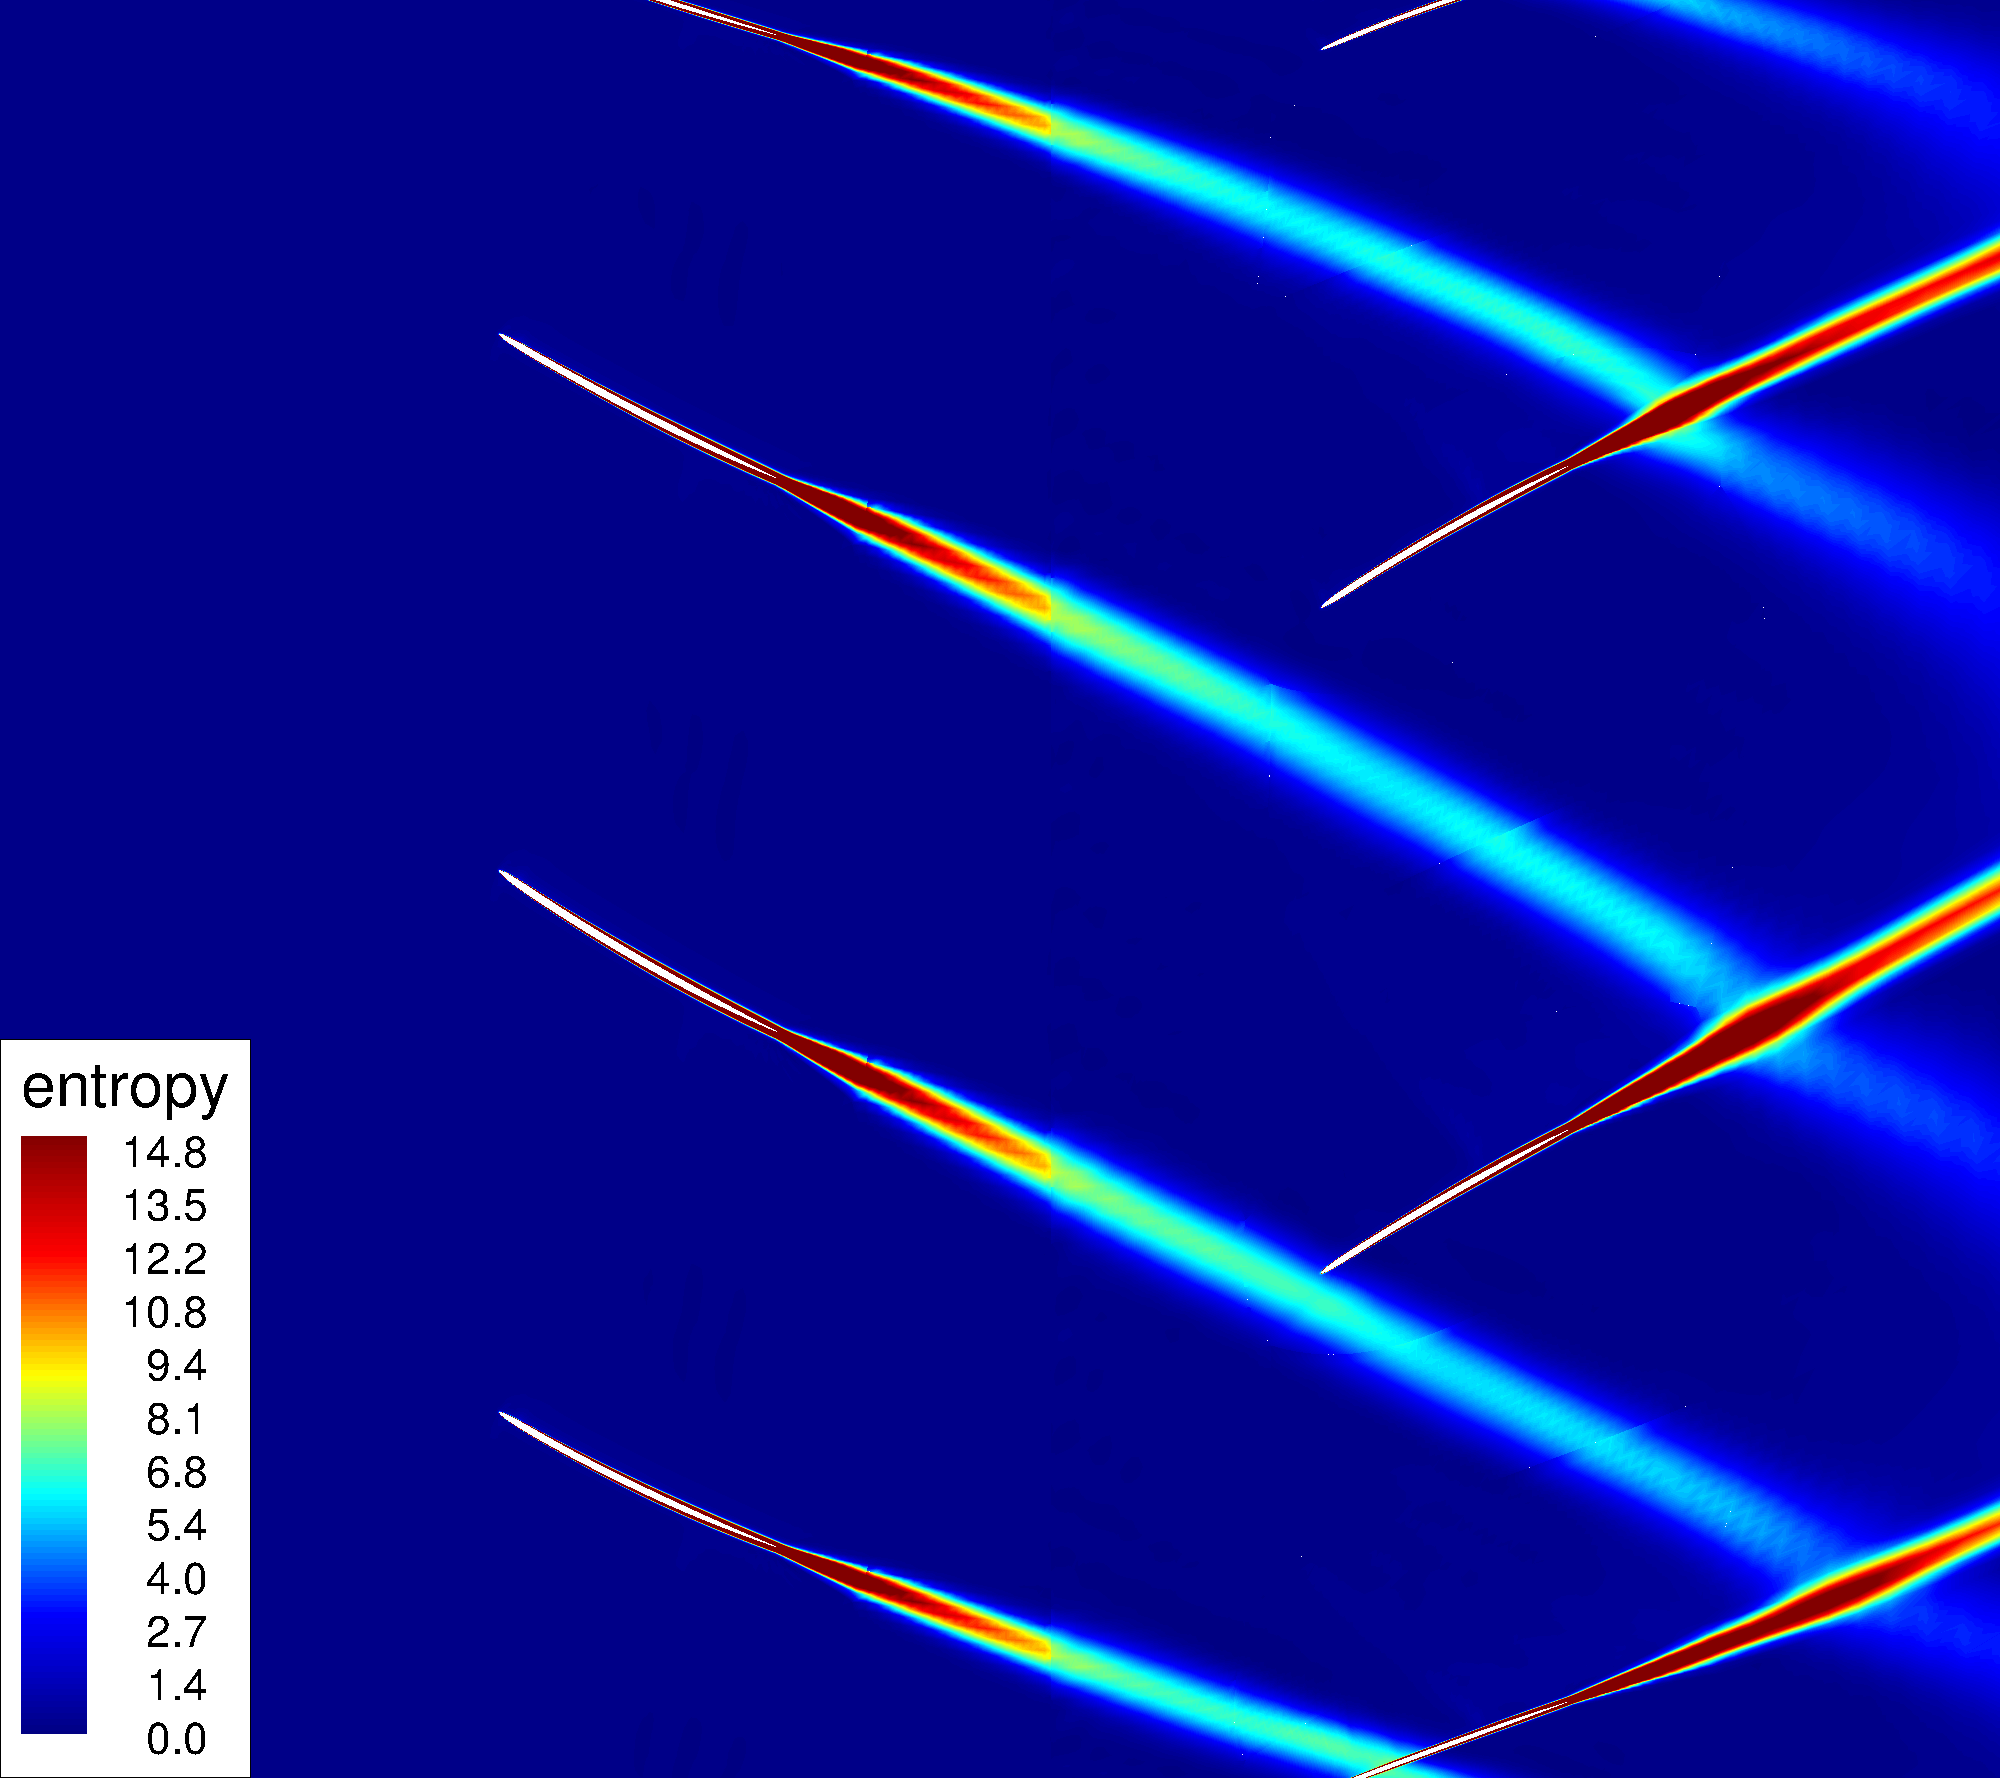
\includegraphics[width=.3\textwidth]{DREAM_HS_TSM_N7_roe2_sa_slice_r_75_entropy.png}
  \caption{High-speed isolated configuration: analysis of the number of harmonics
  required to capture the wake at a 75\% height radial cut.}
  \label{fig:dream_hs_hb_slice_r_conv}
\end{figure}
